\documentclass[12pt,a4paper]{article}
\usepackage{amsmath}
\usepackage{amsthm}
\usepackage{geometry}
\usepackage{enumitem}
\setitemize{noitemsep}
\usepackage{tabularx}
\usepackage{setspace}
\newcolumntype{x}{>{\centering\arraybackslash}X}


\newtheorem{theo}{Theorem}
\newtheorem{prop}[theo]{Proposition}
\newtheorem{lemma}{Lemma}

\usepackage{fontspec,xunicode}
\defaultfontfeatures{Mapping=tex-text}
\setsansfont{TeX Gyre Heros}
\setromanfont{Heuristica}

\usepackage{unicode-math}
\setmathfont{TeX Gyre Schola Math}

\usepackage[backend=biber,style=ext-authoryear-comp,natbib=true,maxbibnames=100,sorting=nyt,sortcites=true,giveninits=false,uniquename=false,uniquelist=false,isbn=false,doi=false,useprefix]{biblatex}

\addbibresource{grouprec.bib}

\usepackage{color,graphicx,setspace}
\newcommand{\mm}[1]{{\color{red} #1}}
\usepackage[normalem]{ulem} % for using strike out with \sout

% removes "in:"
\renewbibmacro{in:}{%
  \ifentrytype{article}{}{\printtext{\bibstring{in}\intitlepunct}}}
% issue number in parentheses
\usepackage{xpatch}
% No dot before number of articles
\xpatchbibmacro{volume+number+eid}{%
  \setunit*{\adddot}%
}{%
}{}{}
% Number of articles in parentheses
\DeclareFieldFormat[article]{number}{\mkbibparens{#1}}

\DeclareFieldFormat*{title}{#1}
\DeclareFieldFormat{titlecase}{\MakeSentenceCase{#1}}
\DeclareFieldFormat[article]{titlecase:journaltitle}{\mkbibitalic{#1}}

% End of bibliography stuff

\usepackage{titlesec} %Package for adjusting the fonts of the \section and \subsection and so forth.
\titleformat{\section}{\Large\bfseries\sffamily}{\thesection.}{1em}{}
\titleformat{\subsection}{\large\bfseries\sffamily}{\thesubsection.}{1em}{}
\titleformat{\subsubsection}{\normalsize\bfseries\sffamily}{\thesubsubsection.}{1em}{}

\onehalfspacing

\begin{document}
\global\long\def\bpi{\bar{p}}%
\global\long\def\upi{\underline{p}}%



\section{Introduction}

Various comments and TODOs:

\begin{itemize}
    \item Discrepancy between the literature on groups, including intergroup conflict parochial altruism, and the experimental literature. The literature considers rich groups, with layers of intra and intergroup interactions. But the experiments show that minimal groups trigger group psychology. We offer an evolutionary explanation for how group cognition can evolve out of a minimal group setup. (Need to check this is fair to the theoretical lit)
    \item Possibly field evidence from segmented societies: me and my brother against my cousin, me and my cousin against the rest of the clan, etc. Shows that the psychology is flexible.
    (DONE)
    \item Many models assume that the cognitive machinery is already there. 
    \item Mention that the "group structure"/"common fate" explanation is
    common sense and may explain some group cooperation.
    \item Mustn't claim our model explains everything in real world conflicts
    \item Model can even explain the evol. of group categorization (i.e. cognition), 
      since selfish types don't need to even observe group labels.
    \item In discussion: why can't a direct reciprocator outcompete? Possible
    answers: can't individuate outgroup members (cf Fearon  Laitin); don't
    regularly interact with any one individual.
\end{itemize}


Humans categorize people into groups, hold attitudes and stereotypes towards
outgroups, and discriminate against them 
\parencite{brewer1985psychology,neuberg2008intergroup}. They also reciprocate 
towards groups, targeting bystanders for the actions of their fellow group members. 
This group psychology may feed into intergroup conflicts between clans, 
ethnicities and nations \parencite{horowitz1985ethnicgroups,
horowitz2001thedeadly,haushofer_both_2010}. It is a puzzle how group psychology 
can evolve. Here we offer an answer.

Previous work on this topic has examined "parochial altruism". These models have 
two limitations. First, they typically
feature just two groups. This lets them explain ingroup altruism and cooperation,
but by definition prevents them addressing phenomena where people treat 
different outgroups differently, including stereotyping and intergroup conflicts.

Second, the models usually impose strong assumptions on group structure: groups
may cooperate together, engage in prespecified forms of intergroup conflict, and/or 
mate assortatively within the in-group. Those assumptions may be realistic
in evolutionarily relevant environments such as hunter-gatherer bands. 
But they fail to explain a key feature of human group psychology: it is flexible. 
That is, human group psychology can
be easily activated or retargeted, even in the absence of long-run cooperation
or conflict. This was the lesson of the original minimal group paradigm in the 
1970s. Previous work had suggested that "common tasks" or a "common fate" were
necessary for group psychology, but \cite{tajfel1971social} 
showed that discrimination and prejudice could be evoked by "minimal" groups, 
based on nothing more than preference for a painting, overestimating the number 
of dots on a screen, or a coin flip. In evolutionary psychology, 
\cite{kurzban2001can} showed that subjects stop categorizing others by race if
it is overruled by other markers of coalition membership, like clothing and 
verbal cues. In the field, segmented societies feature flexible coalitions,
in which minor lineages divide over local issues but unite to oppose a 
rival clan \parencite{fortes2015african}.

Our model avoids these problems. It has an arbitrary number of groups. Groups
do not determine the interaction structure: everyone interacts with
everyone else. Nor do they affect mating or evolution: mating is random,
fitness affects reproduction across the whole population, and children are
rematched randomly into new groups. The cognitive requirements of the model
are also quite minimal. Individuals can learn other individuals' group membership, 
and they can recall others' past behaviour towards them. In short, groups are 
just arbitrary labels.

As it turns out, this minimal structure is enough for intergroup reciprocity to evolve
in a finitely repeated prisoner's dilemma. Group reciprocal types, who cooperate
with someone from group G based on how many people from group G previously cooperated
with them, can have higher fitness. The equilibrium features a mix of group reciprocal
and selfish types.

Group reciprocity involves three capabilities: recording an outgroup's "image"
(its members average level of previous cooperation), categorizing individuals
as outgroup members, and acting towards them on the basis of these two pieces of
information. So, group reciprocity can be a basis for the evolution of outgroup 
categorization, outgroup "image scoring", and discrimination. \cite{fiske2007universal}
argue that humans categorize both individuals and groups on two basic dimensions, 
"warmth" and "competence"; group reputation in our model corresponds to the "warmth" dimension.
There is an analogy here with the literature on individual indirect reciprocity. Models
of "image scoring" or "standing", e.g. \cite{nowak2005evolution},
require individuals to keep track of other individuals' standing, allowing the 
evolution of moral norms and reputations. The same holds here but at group level.

Group reciprocity is also related to generalized upstream reciprocity 
or "paying it forward" \parencite{boyd1989evolution,nowak2007upstream}. The 
literature has concluded that it is hard for 
generalized upstream reciprocity to evolve except in special circumstances. In
our model, a bounded form of generalized upstream reciprocity can evolve, 
because reciprocal cooperation between groups provides an evolutionary advantage
to those groups. Without groups, generalized upstream reciprocity does not allow
for this kind of group selection argument. Possibly, observed cases
of generalized upstream reciprocity 
\parencite[e.g.][]{mujcic2018indirect,yuan2019gift} may involve elements 
of group reciprocity.

The capacity for group reciprocity may also have been a stepping stone in the evolution 
of human cooperation at scale. Interethnic 
peace may be sustained by the threat of reciprocation. This could have allowed
humans to live in peace with neighbouring groups (perhaps punctuated by episodes of
punitive conflict), whereas chimpanzees always attack neighbouring bands on 
contact \parencite{wrangham2012intergroup}. Group reciprocity could also enable 
deeper forms of intergroup cooperation, such as trade.

Here is the logic behind our result. Groups of group-reciprocators
establish cooperative relationships with other groups of group-reciprocators,
while they defect against groups of selfish types. So, when some people are 
group reciprocators, individual fitness depends on one's group's reputation. Group 
reciprocators contribute to this reputation, which is a group-level public good. 
Thus being a group reciprocator is good for the group but costly for the individual. 
This then gives rise to a standard intrademic group selection model, where the 
group-level advantages balance out the individual-level costs 
\parencite{wilson1983group,wade1978critical}. Selfish free-riders within a group 
of mostly group-reciprocators get the highest payoff, but this is balanced
out because most selfish types are in mostly-selfish groups, who have too
few reciprocators to sustain intergroup cooperation.

We use computations to check the robustness of our theoretical model. Our
results confirm that even with relatively rare interactions, group reciprocity can evolve.

Our model also suggests some insights
about how group reciprocal motivations are shaped by evolutionary pressure. The 
most robust forms of group reciprocity have high thresholds of cooperation - that is,
reciprocators only cooperate with groups a high proportion of whose members previously
cooperated towards them. These high thresholds make it less likely that selfish
free riders will invade, since only groups which are almost all reciprocators
get the benefit of mutual cooperation. The resulting equilibrium is 
fragile: it sustains a high level of cooperation, but is also sensitive 
to small amounts of defection.

\section{Literature review}


\cite{tooby2010groups} consider the evolution of human group psychology. In their
theory, groups are coalitions driven by exchange of benefits. In turn,
intergroup relations, including aggression, involve bargaining for resources.
The within-group collective action problem is solved by an advanced coalition 
psychology, including detection of free-riders. This theory predicts that 
human group psychology will be activated for groups which are perceived as 
potential coalitions. One open question is whether this mechanism can explain
the observation that humans exhibit group psychology even in response to
"minimal" stimuli \cite{dunham2018mere}.

Here, we show that intergroup reciprocity can evolve even under "minimal" 
conditions: groups which are arbitrary, with no special mechanisms for in-group
cooperation, collaboration, or resource sharing, no within-group mating and no
explicit group conflict over resources. Even under these conditions, from an 
initial position where people are selfish free-riders, groups who start to act 
reciprocally towards other groups can establish intergroup cooperation and gain 
a fitness advantage. 

We don't think of group reciprocal behaviour as invoking a single specialized 
mental module. Instead, we suggest it involves multiple faculties: categorizing 
people as outgroup members; recording members' actions and combining them into a 
group-level "image score"; motivations to respond reciprocally to outgroup 
members on the basis of the score. Because of this, group reciprocity provides
a pathway for these phenomena to evolve.

Several experiments show evidence for group reciprocity, also known as "vicarious
revenge" \parencite{lickel_vicarious_2006,gaertner2008whenrejection,stenstrom_roles_2008,hugh2017intergroup,hugh2019humans,romano2022direct}. There is also field 
evidence of reciprocity in violent intergroup conflict \parencite{haushofer_both_2010}.
Anthropologists have recorded feud institutions, where group reciprocity is a
normative expectation and where there may be collective mechanisms for managing 
and adjudicating feuds \parencite{boehm1984blood,chagnon1988lifehistories}. 




While there
are evolutionary theories to explain individual reciprocity and revenge
\parencite{mccullough2013cognitive}, there is none for group reciprocity. This is
a problem, because one can't simply assume that the same forces are behind the evolution of 
individual reciprocity and group reciprocity 
\parencite{pietraszewski2013elementary,mccullough2013putting}. 

Group reciprocity is a form of ``upstream reciprocity", where an individual
who is helped or harmed by someone becomes more likely to respectively help 
or harm other third parties \parencite{boyd1989evolution}. It is thought hard 
for upstream reciprocity to evolve,
because it does not target reciprocity in a way that might lead to stable 
bilateral relationships \parencite{nowak2007upstream}.\footnote{By contrast,
we have satisfying theoretical explanations for why group membership might
matter for "downstream" or "indirect" reciprocity, where people help someone
who previously helped others. In particular, group membership may act as a 
"container" for this kind of reciprocity, because fellow group members
expect to interact often in future, or because coalitions are valuable
resources worth defending by third-party punishment
\parencite{yamagishi2000thegroup,romano2022direct,delton2017psychology}.} Indeed,
there is only mixed experimental evidence for upstream reciprocity, with
several papers finding it absent or transient \parencite{ben2004reciprocity,stanca2009measuring,van2016indirect,horita2016transient,greiner2005indirect}. We show that the 
existence of groups makes this problem easier, by allowing 
different \emph{groups} to form bilateral relationships. Group reciprocity 
allows groups to enter mutually beneficial cooperative relationships, achieving 
a fitness advantage. This group selection logic does not apply when reciprocity is 
targeted at the whole population.

\textcite{columbus2023parochial} argue informally that group reciprocity can
be supported by reputation mechanisms at group and individual level. Groups
have an interest in appearing "tough", i.e. able to reciprocate harms; individuals
who reciprocate on behalf of their group may gain an individual reputation for
toughness and (parochial) prosociality. We agree that these mechanisms can enhance
group reciprocity, but we note that they aren't necessary. As we show below,
group reciprocity evolves even when groups don't possess any power of collective 
action (for instance, they can't collectively decide to sanction outgroups, or 
force their members to behave a certain way). Simply making individuals' group 
membership visible is enough to let group reciprocity evolve. We also don't require
group membership to be heritable: in the model, groups are reformed at random
after every generation. This is a strength of the theory because evidence shows 
that humans can quickly perceive and form coalitions even among strangers 
\parencite{tajfel1971social,kurzban2001can,tooby2010groups}.

The logic of group reciprocity does not only explain group reciprocal motivations.
An essential part of any group reciprocal model is that individuals keep mental 
accounts of groups' previous behaviour, in some aggregate form. This mental
accounting provides an evolutionary explanation for why humans hold intergroup 
attitudes \parencite{brewer1985psychology,kurzban2001can}. One simple descriptive 
framework is that groups, like individuals, are perceived on the two dimensions of
warmth and competence \parencite{fiske2007universal}. Our model captures
the warmth dimension. It also shows why a group-level measurement can be cognitively
as important as individual-level characteristics: when humans are group-reciprocators,
aggregated group characteristics (how often that group has cooperated
with your group, and vice versa) predict individual behaviour better than individual
characeristics (how often you have cooperated with this individual).

\textcite{fearon1996explaining} use a repeated-game framework, with 
two classes of possible equilibria, to explain how
different ethnic groups can live at peace. In their "spiral regime", defection
by any member of ethnic group A towards a member of B leads to subsequent 
defection by all members of B towards members of A for a fixed number of periods.
This is an infinitely repeated game with multiple equilibria. The goal is to explain
institutions which support interethnic cooperation; the spiral regime is analogous
to institutions like feuds. Our theory has a different setup and motivation. 
We examine the evolutionary stability of different types in a finitely-repeated game. 
In Fearon and Laitin, cooperation is supported by the threat of collective 
punishment. In our model, group reciprocity is evolutionarily stable because 
individual free-riding is balanced against group selection. So, our model
is designed to explain the evolution of "strong" reciprocal
motivations in humans \parencite{gintis2000strong}, rather than the 
stability of institutions supporting interethnic peace. Ultimately, it is an 
empirical question whether intergroup peace and conflict are best explained 
by rational-actor models, psychological models with "strong" reciprocity,
or a combination of both.

\section{Model}

We consider a mixed population of \mm{size $N$ that is composed of }two types, selfish and group reciprocators (GR). At the beginning of each generation, the population randomly divides into \sout{a large number of} \mm{$G$} groups of size~\mm{$n$} each \mm{(so that $N=nG$)}.
Let~$p$ denote the population share of GR types. 
Let\sout{~$p_g$ be the proportion} \mm{$l_g$ be the number} of GR in group~$g$.\sout{, which is distributed binomially.}

At every step~$t$, everybody interacts with everybody. In each pair, each individual chooses between cooperation and defection. Cooperation entails a cost~$c$ to the cooperator and a benefit~$b$ to her partner. Defection carries no costs. That is, each pair plays the following Prisoner's Dilemma game:
\begin{center}
    \begin{tabularx}{0.5\textwidth}{|x|x|x|}
        \hline
        &   Cooperate   &   Defect  \\
        \hline
        Cooperate   &   $b-c$   &   $-c$    \\
        \hline
        Defect  &   $b$ &   $0$   \\
        \hline
    \end{tabularx}
\end{center}

Selfish types always defect. A GR individual~$i$ starts by cooperating, and then cooperates with all individuals belonging to group~$g$ with a probability~$\phi(l_{gi})$, where~$l_{gi}$ is the \sout{proportion} \mm{number} of individuals from group~$g$ who cooperated with individual~$i$ in round $t-1$.
$\phi(\cdot)$ is monotonically weakly increasing. We consider the cutoff strategy: 
$$
    \phi(l_{gi}) =
    \begin{cases}
        1   &   \text{if } l_{gi} \geq k  \\
        0   &   \text{otherwise.}
    \end{cases}
$$

Equilibrium in this game is as follows: in period 1, group reciprocators help
everyone. In period 2, all group reciprocators help those in ``supraliminal"
groups with $l_g \geq k$. In periods 3 and above, group reciprocators in supraliminal
groups help those in supraliminal groups; they defect against everyone else,
and all other individuals defect.

The fitness is the payoff at the limit where~$t\to\infty$. Equivalently, since the game always settles to a stationary action profile, it is the average payoff of~$T$ rounds when~$T\to\infty$. 

%
Individuals' fitness therefore depends only on whether they are in a ``supraliminal" group, and on their type. Let~$q$ be the 
proportion of supraliminal groups. Let~$\bpi$ be the proportion of 
GR individuals in supraliminal groups (out of the total population in such groups). Let~$\upi$ be the proportion of GR individuals in subliminal groups (out of the total population in such groups). It follows that
\begin{itemize}
    \item Group reciprocators in supraliminal groups get a payoff of~$(\bpi qb - qc)\mm{N}$ \mm{$= \Sigma_{\{g|l_g \geq k\}}[l_gb-nc]$}.
    \item Selfish types in supraliminal groups get~$\bpi qb\mm{N}$ \mm{$= \Sigma_{\{g|l_g \geq k\}}l_gb$}.
    \item Group reciprocators and selfish types in subliminal groups get~$0$.
\end{itemize}

After each generation, reproductive success is proportional to fitness, the total population size stays the same, and children are remixed randomly into new groups of the same size.
%
The mean fitness of the GR type is

\begin{equation*}
\frac{
  \bpi q(q(\bpi b - c))\mm{N}
}{
  p
}
\mm{=\frac{\Sigma_{\{g|l_g \geq k\}}l_g \Sigma_{\{g|l_g \geq k\}}[l_gb-nc]}{\Sigma_gl_g}}
\end{equation*}

and the mean fitness of selfish types is

\begin{equation*}
\frac{
  (1 - \bpi)q(q\bpi b)\mm{N}
}{
  1 - p
}
\mm{=\frac{\Sigma_{\{g|l_g \geq k\}}(n-l_g) \Sigma_{\{g|l_g \geq k\}}l_gb}{\Sigma_g(n-l_g)}}
\end{equation*}

After rearranging, the mean fitness of reciprocators is higher if


\begin{equation}
\label{gr-wins}
\frac{ \bpi - p}{ 1 - p} \ge \frac{c}{b}
\mm{\Longleftrightarrow \frac{N\Sigma_{\{g|l_g \geq k\}}l_g-M\Sigma_gl_g}{N-\Sigma_gl_g} \ge M\frac{b}{c}}.
\end{equation}

where \mm{$M \equiv qN=\Sigma_{\{g|l_g \geq k\}}n$ and 

\[
\bpi = \frac{\Sigma_{\{g|l_g \geq k\}}l_g}{M}
\]}

\begin{prop}
\label{prop:decrease_in_p}
    \mm{If $M \neq \emptyset$, then} the LHS of equation \eqref{gr-wins} is decreasing in $p=\mm{\frac{\Sigma_gl_g}{N}}$ \sout{and is equal
to the threshold $k$ when $p = 0$}.\footnote{\sout{
    When the share of GR in the population is very small, the probability that $p_g = k$ conditional on~$p_g\geq k$ goes to one.
}}
\end{prop}

\begin{proof}
    See Appendix.
    
    \mm{
    First rewrite the LHS of \eqref{gr-wins} as follows: $LHS=M-Nx$, where $x \equiv \frac{\Sigma_{\{g|l_g \geq k\}}(n-l_g)}{N-\Sigma_gl_g}$ is the proportion of selfish types who belong to supraliminal groups.
    A marginal increase in $p$ is modeled by a random selection of a selfish type who is replaced by a GR-type. That is, with probability $x$ this selfish type belongs to a supraliminal group and otherwise it belongs to a subliminal group.

    Suppose first that the group from which the selfish type is randomly selected cannot switch from being subliminal to being supraliminal (even if was of size $l_g=k-1$).\footnote{\mm{What we mean by that is that this group will not be included in the sum $\Sigma_{\{g|l_g \geq k\}}$ even if it becomes of size $k$.}}
    Then, with probability $x$, the increase in the LHS is given by $-N(\frac{\Sigma_{\{g|l_g \geq k\}}(n-l_g)-1}{N-\Sigma_gl_g-1}-x)$, and with probability $1-x$ the increase in the LHS is given by $-N(\frac{\Sigma_{\{g|l_g \geq k\}}(n-l_g)}{N-\Sigma_gl_g-1}-x)$.
    Therefore, the expected increase in the LHS is given by
    \begin{equation*}
        -N[x(\frac{\Sigma_{\{g|l_g \geq k\}}(n-l_g)-1}{N-\Sigma_gl_g-1}-x)+(1-x)(\frac{\Sigma_{\{g|l_g \geq k\}}(n-l_g)}{N-\Sigma_gl_g-1}-x)] 
    \end{equation*}
    \begin{equation*}
        =-N\big[\frac{x[\Sigma_{\{g|l_g \geq k\}}(n-l_g)-1]+(1-x)\Sigma_{\{g|l_g \geq k\}}(n-l_g)}{N-\Sigma_gl_g-1}-x \big]
    \end{equation*}
    \begin{equation*}
        =-N\big[\frac{\Sigma_{\{g|l_g \geq k\}}(n-l_g)-x}{N-\Sigma_gl_g-1}-x \big].
    \end{equation*}

    Recalling that $x=\frac{\Sigma_{\{g|l_g \geq k\}}(n-l_g)}{N-\Sigma_gl_g}$ we get that
    \begin{equation*}
       -N\big[\frac{\Sigma_{\{g|l_g \geq k\}}(n-l_g)-x}{N-\Sigma_gl_g-1}-x \big]= -N\big[\frac{x(N-\Sigma_gl_g)-x}{N-\Sigma_gl_g-1}-x \big]=0.
    \end{equation*}
   That is, if we do not allow groups to switch from being subliminal to being supraliminal, then the effect of randomly replacing a selfish type with a GR-type on the LHS is zero. However, if this replacement results in a subliminal group becoming supraliminal (note that the opposite change is impossible), then $x$, the proportion of selfish types who belong to supraliminal groups, necessarily increases (there will be more selfish types in supraliminal groups out of less selfish types in the population), implying that $M-Nx$ (the LHS) must decrease.
            }
\end{proof}

It follows that there is a unique ESS with a positive share of group
reciprocators if and only if $k > \frac{c}{b}$. Otherwise the population is homogeneously selfish in the unique ESS.

\section{Simulations}

The model includes two simplifying assumptions: a large number of groups, and a large
number of rounds $T$ in each generation. To check how these simplifications affect
the result, we run simulations. We use the following sets of parameters:
$c/b = 0.2, 0.5$; $T = 10, 20$; N groups = $10, 50$; $k = 0.4, 0.8$. This gives
16 unique combinations of parameters. We always set $G = 8$ and start with
half the population as GR types. Fitness is normalized so that the "sucker's payoff"
$-c$ equals zero. For each combination we run 20 experiments, 
each lasting 500 generations. After 500 generations we record the proportion of 
group reciprocators. 

Figure \ref{fig:sims} shows the mean proportion of GR types across all experiments for
each combination of parameters. For all combinations of parameters but one,
either GR types or selfish types always went to fixation within 500 generations. In
these cases, the proportion of GR types is just the proportion of experiments
where GR types went to fixation.

A shorter number of periods $T$ leads to fewer 
GR types, as expected since it gives more weight to the early-round losses of GR 
types. The number of groups does not seem to affect the evolution of GR types. As
expected, a higher cost-benefit ratio $c/b$ leads to fewer GR types. A higher 
threshold $k$ also usually leads to more GR types, and in particular when 
$k < c/b$, group reciprocity never evolves. One exception is with 50 groups
and $T = 20$: in this case, more group reciprocators evolve when $k = 0.4$. 
This is also the sole parameter combination where not all experiments went to 
fixation.


In our analytic result with many groups, group size $G$ doesn't matter. 
With finite numbers of groups, all groups may fall below the $k$-threshold in a
given generation. This becomes more likely when $G$ is large and when the
population proportion of GR types is below the threshold (because when $G$ is
large, the proportion of GR types in each group becomes concentrated on
the population proportion). So, group size may matter. We ran one further 
parameter set to check whether group reciprocity could be
stable in larger groups. We set $G =  40$, N groups = 40, $T = 20$, $k = 0.6$ 
and $c/b = 0.1$. In 10 experiments, the proportion of group reciprocators was
always between 60 and 70 per cent after 500 generations. So, evolution of
group reciprocity is possible even with large groups, although it seems to 
require high benefit-cost ratios.


\begin{figure}[h]
  \caption{Simulation results. Plots show proportions of group reciprocator types after 100 generations.}
  \label{fig:sims}
  \centering
    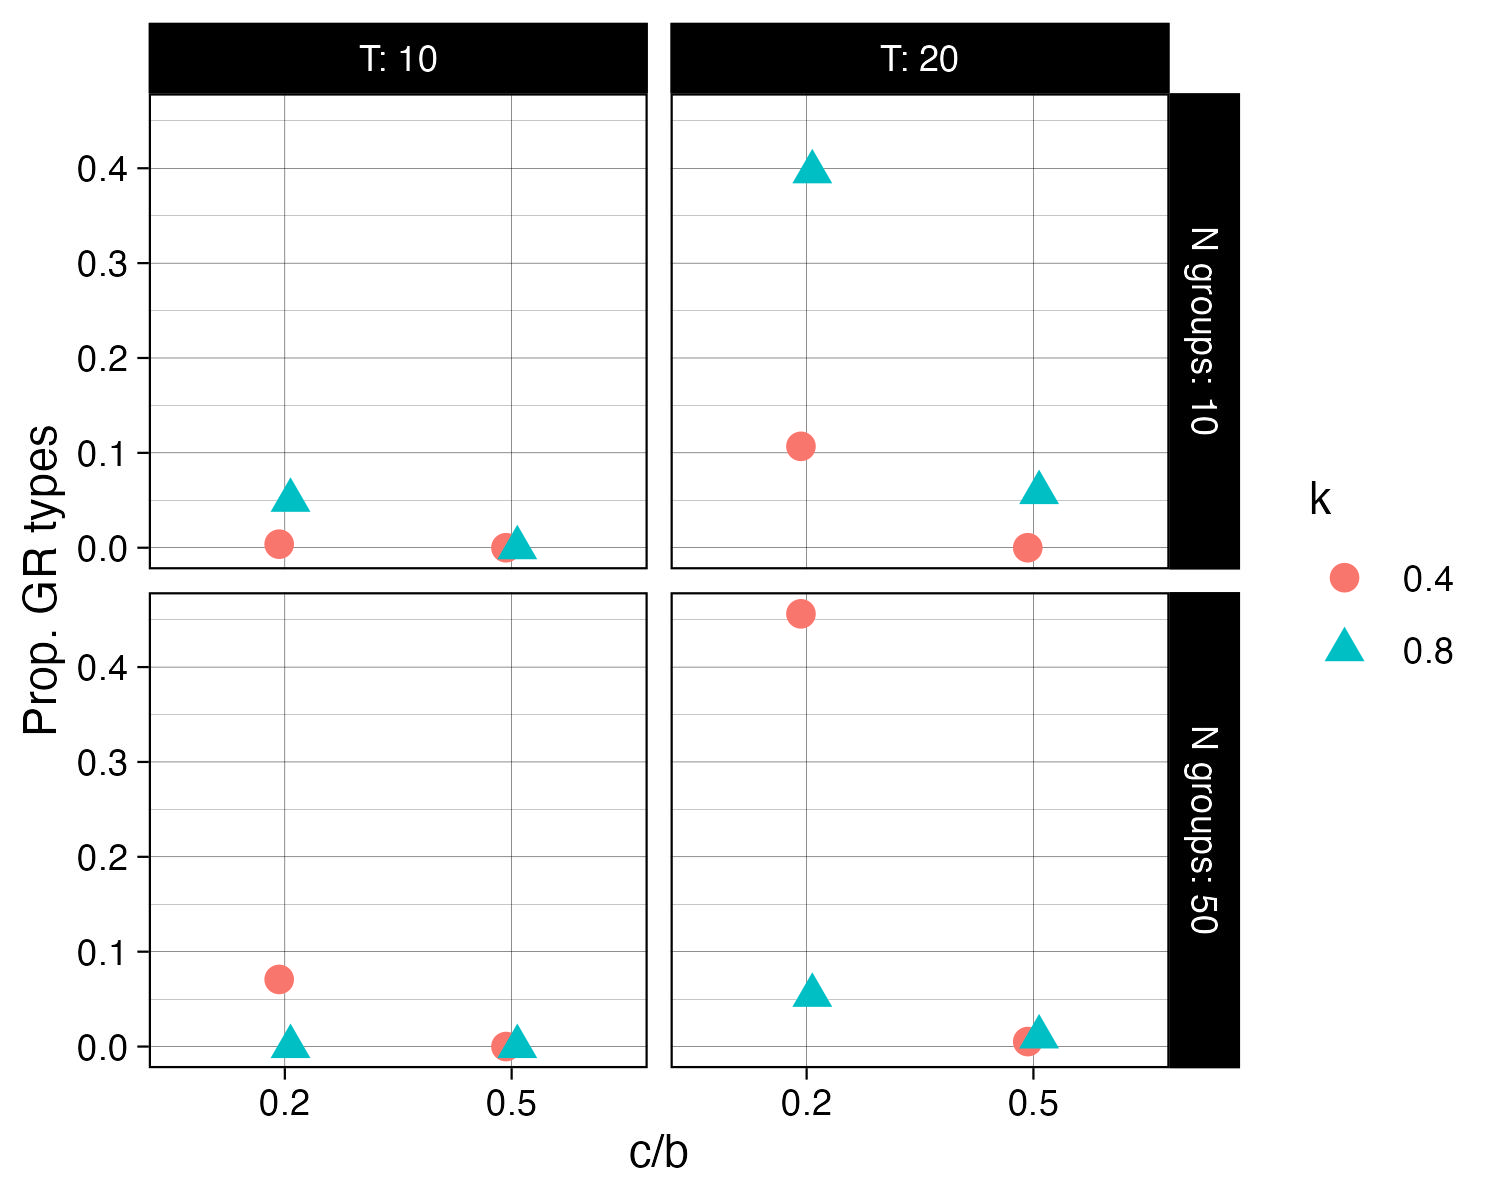
\includegraphics[height=4in]{R files/basic-experiment.jpeg}
\end{figure}

\section{Conclusion}

We introduced an evolutionary model of group reciprocity. Group reciprocal 
motivations can evolve under plausible parameter values for human populations 
[XXX can we say that?]. Evolved group reciprocity could explain why humans
track group-level reputations. It also provides a simple way that upstream
reciprocity can evolve. 

The simplest alternative theory of group reciprocity is perhaps that many groups
are able to solve collective action problems, i.e. to incent or persuade
their members to maximize the payoff of the group. If so then reciprocity 
towards other groups could be optimal in the same way as individual-level
reciprocity. Lab experiments show group reciprocity even among "minimal" groups 
which have no way to address collective action problems. But this might be
because participants over-generalize, bringing into the lab their intuitions 
about behaviour that makes sense in the field. A useful next step would be to
examine group reciprocity in the field, among groups which lack institutions
for collective action.

\printbibliography


\newpage
\appendix
\renewcommand*\thetable{\Alph{section}.\arabic{table}}
\renewcommand*\thefigure{\Alph{section}.\arabic{figure}}
\setcounter{figure}{0}
\setcounter{table}{0}
\setcounter{equation}{0}
\numberwithin{equation}{section}
\section{Proofs}
\label{sec:proofs}
\subsection{Proof of Proposition \ref{prop:decrease_in_p}}
We will first prove an auxiliary lemma and then the main result.
\begin{lemma}
\label{lemma:eqiv_formulation}
Let $x_1,x_2,...,x_n$ be iid Binomially-distributed variables with probability of success $p$, and let $x_i=1$ denote the event where $x_i$ fails. Then showing that $\frac{ \bpi - p}{ 1 - p}$ decreases in $p$ is equivalent to showing that $\frac{p(x_1=1|S_n \leq k)}{p(x_1=1)}$ increases in $p$, where $S_n=x_1+x_2+...+x_n$.
\end{lemma}
% \noindent \textbf{Proof of Lemma \ref{lemma:eqiv_formulation}}
\begin{proof}
First note that proving that the LHS of \eqref{gr-wins} is decreasing in $p$ is equivalent to proving that $1-\frac{ \bpi - p}{ 1 - p} = \frac{ 1- \bpi}{ 1 - p}$ is increasing in $p$. Second, note that 
% if $p$ is the probability of success of a Binomially-distributed variable $x_i$, then 
$1- \bpi$ captures the expected proportion of failures of a Binomially-distributed variable given that the proportion of successes was at least $k$, or, put differently, given that the proportion of failures was at most $k$. Finally, we can replace the expected proportion of failures with the probability of a failure. All in all, we get that proving that $\frac{ 1- \bpi}{ 1 - p}$ is increasing in $p$ is equivalent to showing that $\frac{p(x_1=1|S_n \leq k)}{p(x_1=1)}$ is increasing in $p$.
% hence decreasing in $q$.
\end{proof}
\vspace{0.3cm}

\noindent \textbf{Proving the proposition}
\vspace{0.3cm}

\begin{proof}
Lemma \ref{lemma:eqiv_formulation} implies that if $x_i=1$ denotes the event where $x_i$ fails, and $S_n$ counts the number of failures among $n$ trials, then we need to show that $\frac{p(x_1=1|S_n \leq k)}{p(x_1=1)}$ increases in the probability of success $p$.
For tractability, we will now revert to the more standard notation of $x_i=1$ as denoting the event where $x_i$ \textit{succeeds} (s.t. $S_n$ counts the number of successes among $n$ trials), and show that $\frac{p(x_1=1|S_n \leq k)}{p(x_1=1)}$ \textit{decreases} rather than increases in the probability of success $p$.
\vspace{0.6 cm}

\noindent \textbf{Version 1}

\begin{equation*}
    \frac{p(x_1=1|S_n \leq k)}{p(x_1=1)}=\frac{p(s_n \leq k|x_1=1)}{p(s_n \leq k)}=\frac{p(s_{n-1} \leq k-1)}{qp(s_{n-1} \leq k)+pp(s_{n-1} \leq k-1)}
\end{equation*}


\begin{equation*}
    =\frac{p(s_{n-1} \leq k-1)}{q(p(s_{n-1} \leq k)-p(s_{n-1} \leq k-1))+p(s_{n-1} \leq k-1)}=\frac{p(s_{n-1} \leq k-1)}{qp(s_{n-1}=k)+p(s_{n-1} \leq k-1)}.
\end{equation*}


\vspace{0.3 cm}
\noindent \textbf{Version 2}
\vspace{0.6 cm}

$\frac{p(x_1=1|S_n \leq k)}{p(x_1=1)}=\frac{p(s_n \leq k|x_1=1)}{p(s_n \leq k)}=\frac{p(s_{n-1} \leq k-1)}{qp(s_{n-1} \leq k)+pp(s_{n-1} \leq k-1)}$

\vspace{0.3cm}
$=\frac{p(s_{n-1} \leq k-1)}{q(p(s_{n-1} \leq k)-p(s_{n-1} \leq k-1))+p(s_{n-1} \leq k-1)}=\frac{p(s_{n-1} \leq k-1)}{qp(s_{n-1}=k)+p(s_{n-1} \leq k-1)}.$
\vspace{1 cm}

\noindent 
Using a known result,\footnote{See equations (3) and (4) in https://mathworld.wolfram.com/BinomialDistribution.html.} according to which
\begin{equation*}
    p(s_n \leq k) = \frac{n!}{(n-k-1)!k!}\int_0^q t^{n-k-1}(1-t)^k dt = \frac{n!}{(n-k-1)!k!}\int_0^1 q^{n-k} s^{n-k-1} (1-qs)^k ds,
\end{equation*}
we get that $\frac{p(x_1=1|S_n \leq k)}{p(x_1=1)}$ is decreasing in $p$ if and only if $\frac{q \binom{n-1}{k} p^k q^{n-k-1}}{\frac{(n-1)!}{(n-k-1)!(k-1)!}\int_0^1 q^{n-k}s^{n-k-1}(1-qs)^{k-1} ds}$ is decreasing in $q$, i.e., if and only if $\frac{\binom{n-1}{k} p^k}{\frac{(n-1)!}{(n-k-1)!(k-1)!}\int_0^1 s^{n-k-1}(1-qs)^{k-1} ds}$ is decreasing in $q$.
\vspace{0.3cm}
Thus, it is sufficient to show that $\int_0^1 s^{n-k-1}(\frac{1-qs}{1-q})^{k-1}\frac{1}{1-q} ds$ is increasing in $q$. Since $(\frac{1-qs}{1-q})^{k-1}\frac{1}{1-q}$ is non-decreasing in $q$ for every $s \in [0,1]$, the proof is complete.

\end{proof}

\end{document}
%%% THE REST OF THE ATTEMPTS TO PROVE ARE IN THE SEPARATE FILE

\subsection*{Proof that \eqref{gr-wins} goes to $k$ as $p \to 0$}


Consider

\[
\frac{\bpi - p}{1-p}
\]
The limit as $p \to 0$ is given by $\bpi$. For $k=0$ this is
0 since $\bpi = p$. For $k>0$, write
\[
\bpi=\frac{1}{G}\frac{\sum_{l=kG}^{G}l\phi(l,G,p)}{\sum_{l=kG}^{G}\phi(l,G,p)}=\frac{1}{G}\frac{\sum_{l=kG}^{G}l\binom{G}{l}p^{l}(1-p)^{G-l}}{\sum_{l=kG}^{G}\binom{G}{l}p^{l}(1-p)^{G-l}}.
\]

The limit of this is given by L'H\^{o}pital's rule, since the denominator
goes to zero. Differentiating top and bottom gives
\[
\frac{1}{G}\frac{\sum_{l=kG}^{G}l\binom{G}{l}(l-Gp)p^{l-1}(1-p)^{G-l-1}}{\sum_{l=kG}^{G}\binom{G}{l}(l-Gp)p^{l-1}(1-p)^{G-l-1}}
\]
so we have to apply the rule again. Continuing thus we eventually hit:
\[
\frac{1}{G}\frac{kG\binom{G}{l}(l-Gp)(l-1-Gp)(\cdots)(l-kG-Gp)p^{0}(1-p)^{G-2kG}+\cdots}{\binom{G}{l}(l-Gp)(l-1-Gp)(\cdots)(l-kG-Gp)p^{0}(1-p)^{G-2kG}+\cdots}
\]
 where all but the first terms vanish, leaving
\[
\frac{1}{G}\frac{kG\binom{G}{l}(l-Gp)(l-1-Gp)(\cdots)(l-kG-Gp)p^{0}(1-p)^{G-2kG}}{\binom{G}{l}(l-Gp)(l-1-Gp)(\cdots)(l-kG-Gp)p^{0}(1-p)^{G-2kG}}=\frac{1}{G}kG=k.
\]


(Old stuff)

\begin{align}
    q & = & 1 - CDF(G, p') \\
    \bpi & = & E[p_k | p_k \ge c] \\
    \upi & = & E[p_k | p_k < c]
\end{align}

Where $CDF$ is the binomial distribution of $p'$ out of $G$ successes, and
the conditional expectations are also taken according to this distribution.

Computations are in continuous-model-computations.R in dropbox. Plotting
reveals:

When $p$ is sufficiently below $c$, $p' = p$ and group reciprocity is 
selectively neutral, since group reciprocators and selfish types are
almost all in subliminal groups.

For some parameters, and intermediate values of $p$, $p'>p$ so that
group reciprocity is being selected for. That is, some groups successfully
manage to cooperate with other groups and have higher average fitness.

For high enough values of $p$, $p' < p$. This is because when almost everyone
is cooperating, a selfish type is almost surely in a supraliminal group
and benefits by freeriding.

Conjectures and questions.

1. What if the threshold can evolve? Might higher thresholds always 
be beneficial? If so, probably only few group reciprocators exist,
and very few are in supraliminal groups. One way to do this is
generalize the model to have high- and low-threshold types, and see
who wins. Note that in the model as is, a selfish type just has a
"threshold" of above 1. Another approach is to ask if a single
person with a different threshold can invade. He will change the
behaviour of other groups to him, but as there are many groups,
we can ignore the effects on other people's fitness and just
ask if he outcompetes other group reciprocators.
\end{document}
